\documentclass[10pt,aspectratio=149]{beamer}

\usetheme[ku, totalframes=hide, fnolabel=]{Frederiksberg}

%% ----------------------------------
%% display

\usepackage{amsmath} % for better display of equations

% use proper unicode fonts
\usepackage[T1]{fontenc}
\usepackage[utf8]{inputenc}

\DeclareTextSymbol{\degre}{T1}{6}

\usepackage{pgfplots}
\usepackage{pgfplotstable}
\usepackage{tikz}
\usepackage{tikz-cd}
\usetikzlibrary{calc, shapes}
\usetikzlibrary{shapes.geometric,shapes.arrows,decorations.pathmorphing}
\usetikzlibrary{matrix,chains,scopes,positioning,arrows,fit}
\tikzstyle{every picture}+=[remember picture]

\usepackage{graphicx}
\graphicspath{{tex/}}


\setlength{\parindent}{0pt} % remove automatic indent


\definecolor{tcolor}{rgb}{0.07,0.93,0.3}
\definecolor{bcolor}{rgb}{0.25,0.67,0.1}
\definecolor{lightblue}{rgb}{0.15,0.5,0.75}
\definecolor{violet}{rgb}{0.3,0.2,0.55}

\setbeamercolor{alerted text}{fg=orange}
\setbeamerfont{alerted text}{series=\bfseries}



%% ----------------------------------
%     Title and authorship information


\author[]{Isabelle Boulangeat, Matthieu Leblond, Tanguy Daufresne, Dominique Gravel}
\title[]{How vegetation-herbivores feedbacks mediate vegetation transitions?}
% \subtitle{Isabelle Boulangeat}

\date[]{\today}
% \institute{Université du Québec à Rimouski}


\begin{document}

%==========================================================================

\begin{frame}[plain]

\titlepage

\end{frame}


%==========================================================================
%==========================================================================

\begin{frame}{Biomes distribution (Whittaker 1975)}

\centering
\includegraphics[width=.5\textwidth]{../../illustrations/biomes3bis.pdf}\\
\vspace{1em}
Strong effect of the climate but...\\

\end{frame}

%==========================================================================
%==========================================================================

\begin{frame}{Other drivers}


% \begin{quote}
%     ``tree line in mountains may be more influenced by the grazing of seedlings and saplings than most people have supposed'' Grace et al. 2002
%   \end{quote} 
\only<1>{
Treeline is largely influenced by grazing sheep \\
\vspace{2em}
% \begin{itemize}
% \item Experimental studies and observations (Speed \textit{et al.} 2010, 2011, 2012)
% \item 
% \end{itemize}

% \centering
\includegraphics[width=.5\textwidth]{../../illustrations/pelouse_adret_lautaret2.JPG}
\includegraphics[width=.5\textwidth]{../../illustrations/aulnaie_ubac_lauraret.JPG}\\
% \small{Modelisation and simulations in the French Alps (Boulangeat \textit{et al.} 2014)}
}

% \end{frame}
% % 
% %==========================================================================
% %==========================================================================

% \begin{frame}{Forest and savannas}

\only<2>{

Forest-savanna transitions are driven by fire and herbivores \\
\vspace{1em}

\flushleft
\includegraphics[width=.8\textwidth]{../presentations_figs/staver.png}

\flushright
\includegraphics[width=.8\textwidth]{../presentations_figs/holdo.png}
}

% \only<3>{

% \begin{tabular}{m{.4\textwidth} m{.6\textwidth}}

% \includegraphics[width=.4\textwidth]{../presentations_figs/holdo2.png}

% &
% \includegraphics[width=.6\textwidth]{../presentations_figs/holdo3.png} \\
% \end{tabular}

% }

\end{frame}


%==========================================================================

\begin{frame}{Objectives}


What is the effect of $\overbrace{\text{\alert{trophic interactions}}}^\text{wild animals}$ on the distribution of the vegetation?

\vspace{1em}

\begin{columns}
\begin{column}{0.5\textwidth}
\includegraphics[width=\textwidth]{../../illustrations/biomes3bis.pdf}
\end{column}
\begin{column}{0.5\textwidth}

Investigating distributions along the temperature gradient at

\begin{itemize}

\item Treeline ecotone
\item Temperate/boreal forest ecotone
\end{itemize}
\end{column}
\end{columns}

\end{frame}
%==========================================================================

% \begin{frame}{Approach}


% \begin{enumerate}

% \item State transition model (spatially implicit)

% \item Transitions depending on climate

% \item Two-ways trophic interactions

% \end{enumerate}


% \end{frame}
%==========================================================================
%==========================================================================

\begin{frame}{Part 1: Forest-grassland transition}

\only<1>{
\includegraphics[width=0.9\textwidth]{../presentations_figs/3states.pdf}

}

\only<2>{
Proportions of landscape\\
$G$ = Grasslands\\
$S$ = Seedling-dominated\\
$T$ = Forest\\

\begin{columns}
      \begin{column}{0.5\textwidth}


\begin{center}
\tikz[baseline]{\node[draw, circle, anchor=base] (G){G};} \hspace{3em}
\tikz[baseline]{\node[draw, circle, anchor=base] (S){S};} \hspace{3em}
\tikz[baseline]{\node[draw, circle, anchor=base] (T){T};} 
\end{center}
\begin{tikzpicture}[overlay]
\draw[-angle 45] (G.east) -- (S.west) node[midway,below] {$cfT$};
\draw[-angle 45] (S.east) -- (T.west) node[midway,below] {$\alpha$};
\draw[-angle 45] (T.north) to[bend right=50] node[midway,above] {$\delta $} (G.north) ;
% \draw[-angle 45] (T.north) to[bend right=50] node[near end,above] {$\delta cfT$} (S.north) ;
\end{tikzpicture}


\end{column}
      \begin{column}{0.5\textwidth}

\[
\left\{
\begin{array}{r c l}

G &=& 1 - T - S\\

\rule{0pt}{7ex} \frac{dT}{dt} &=& 
\overbrace{\alpha S}^\text{succession} - \overbrace{\delta T}^\text{disturbance}\\

\rule{0pt}{7ex} \frac{dS}{dt} &=& 
\overbrace{fT}^\text{seeds}
\overbrace{cG}^\text{colonisation}
-
\overbrace{\alpha S}^\text{succession} \\

\end{array}
\right.
\]


\end{column}
\end{columns}

}

\end{frame}
%==========================================================================
%==========================================================================

\begin{frame}{Climate effect implementation}

\centering
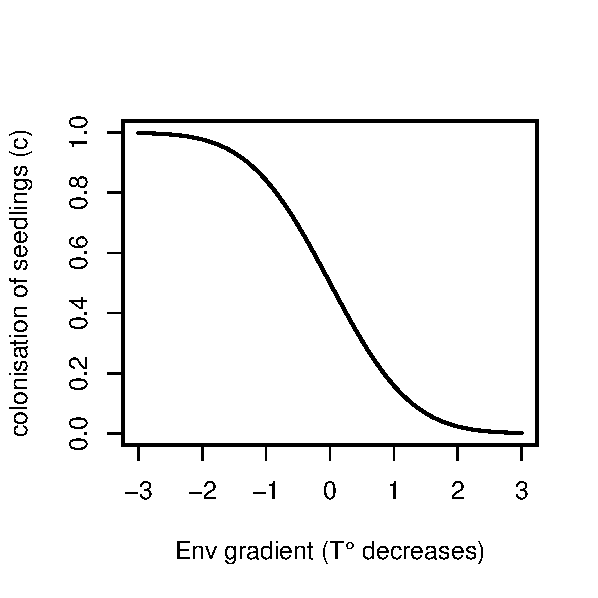
\includegraphics[width=0.5\textwidth]{../../ThreeSTModel/graphs/climate.pdf}
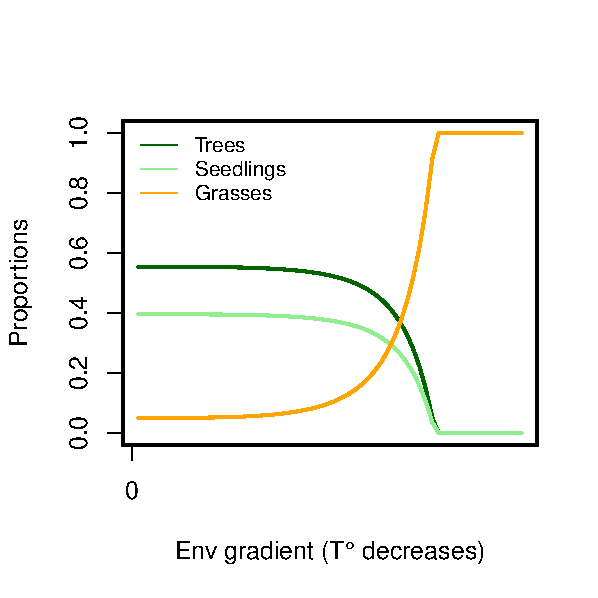
\includegraphics[width=0.5\textwidth]{../../ThreeSTModel/graphs/graphs_vegetDyn.pdf}
  

\end{frame}
%==========================================================================
%==========================================================================

\begin{frame}{Herbivore dynamics}

Based on metaphysiological model Owen-Smith 2002\\

The herbivore dynamic is modelled as a \alert{total biomass}.

%-----
\[
\left.
\begin{array}{r c l}{}

\frac{dH}{dt} &=& 
\overbrace{H*I}^\text{biomass gains} - \overbrace{H*(p+qe^{-zI}+m)}^\text{biomass losses})

\end{array}
\right.
\]

\vspace{2em}

\small{
\begin{tabular}{cl}
$p$ & metabolic attrition rate \\

$q$ & maximum mortality rate due to starvation \\

$m$ & minimum mortality rate when food is abundant \\

$I$ & vegetation intake rate \\
\end{tabular}
}

\end{frame}
%==========================================================================
%==========================================================================

\begin{frame}{Vegetation-herbivore interactions}

\[
I = \overbrace{\frac{\tau R_1}{\mu+R_1}}^\text{intake rate of preferred resource} 
+ \overbrace{\frac{\theta R_2}{\nu+R_2}\frac{1}{1+e^{r(\frac{\tau R_1}{\mu+R_1} - p - m)}}}^\text{intake rate of secondary resource} 
\]

% \centering
% 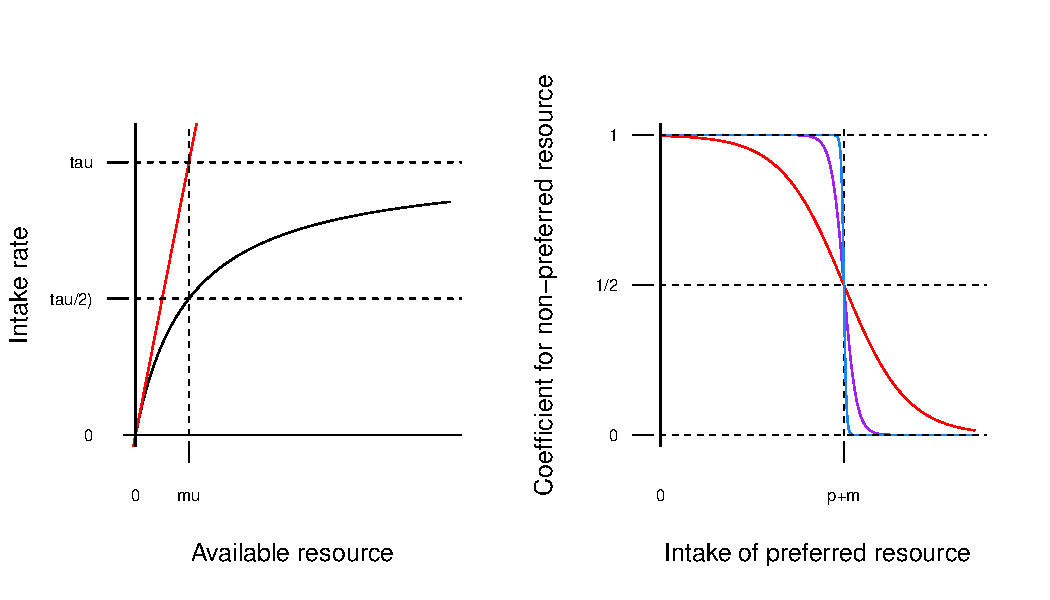
\includegraphics[width=0.7\textwidth]{../graphs/intakes_v1.pdf}
 

\end{frame}
%==========================================================================
%==========================================================================

\begin{frame}{Feedback effects of herbivores on the vegetation}


\vspace{1em}
$\text{Herbivore pressure ($P_G$ and $P_S$)} = \frac{\text{Total intake}}{\text{Available biomass}}$\\
\vspace{1em}

Herbivores impact \alert{colonisation by seedlings (c)} and \alert{succession($\alpha$)}

% 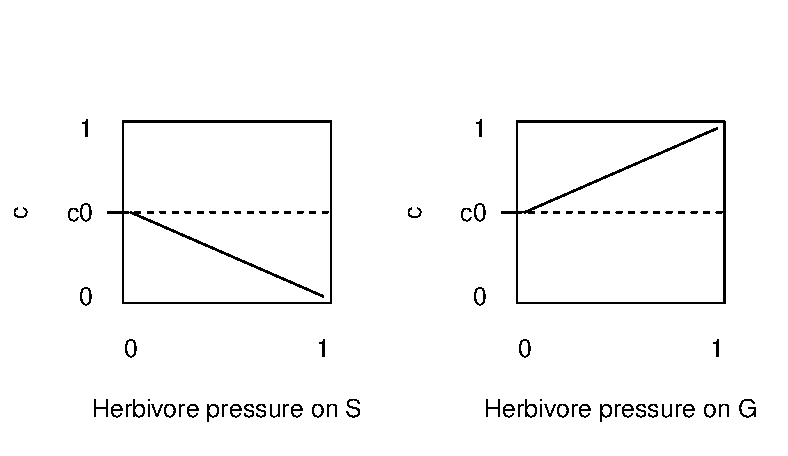
\includegraphics[width=0.6\textwidth]{../graphs/herbPressure_onc.pdf}
% 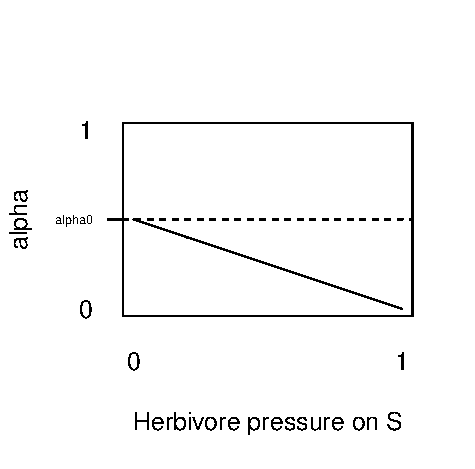
\includegraphics[width=0.35\textwidth]{../graphs/herbPressure_onalpha.pdf}

% \[
% c = f(S, G) = P_G - c_0(P_G+P_S) + c_0
% \]



% \[
% \alpha = f(S, G) = \alpha_0(1-P_S)
% \]


\end{frame}
%==========================================================================
%==========================================================================

\begin{frame}{Assumptions of the analysis}

\centering
\includegraphics[width=0.8\textwidth]{../presentations_figs/3states_2.pdf}

\small{
\begin{itemize}
% % \item Two herbivores: 
% % \begin{itemize}
% % \item A \alert{grazer} eats \alert{grasses} only. \\
% % \item A \alert{browser} prefers \alert{seedlings} but can feed on \alert{grasses} too.\\
% % \end{itemize}

\item The two herbivores have the same demographic parameters

\item Grasses provide 4 times more eatable biomass than seedlings

\item Herbivores \alert{compete}, according to their total biomass, on grass ressource 

\end{itemize}
}

\end{frame}

%==========================================================================
%==========================================================================

\begin{frame}{Steady state analysis}

\only<1>{
Browser vs grazer effect on vegetation distribution
\centering
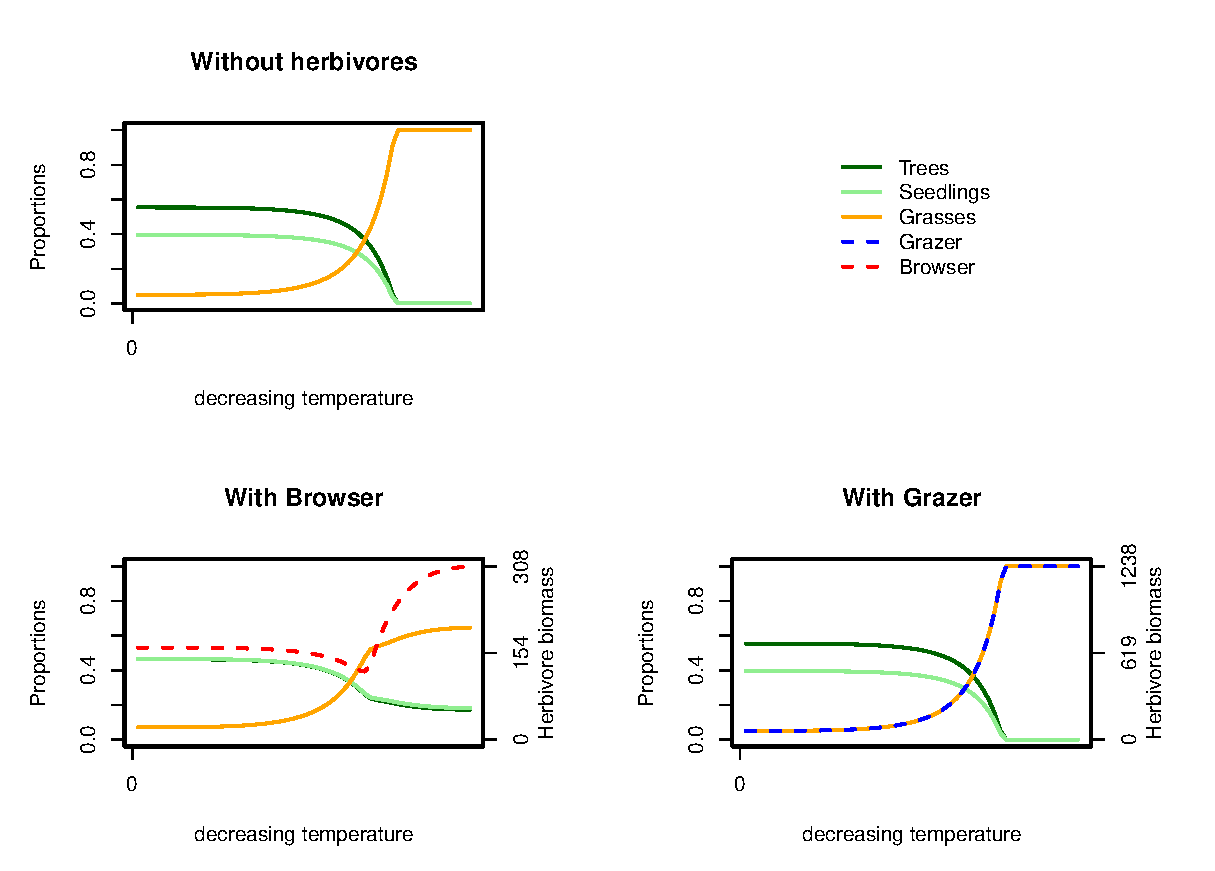
\includegraphics[width=0.8\textwidth]{../../ThreeSTModel/graphs/effectOnVeget_compare.pdf}
}

\only<2>{
Browser vs grazer effect on vegetation distribution
\centering
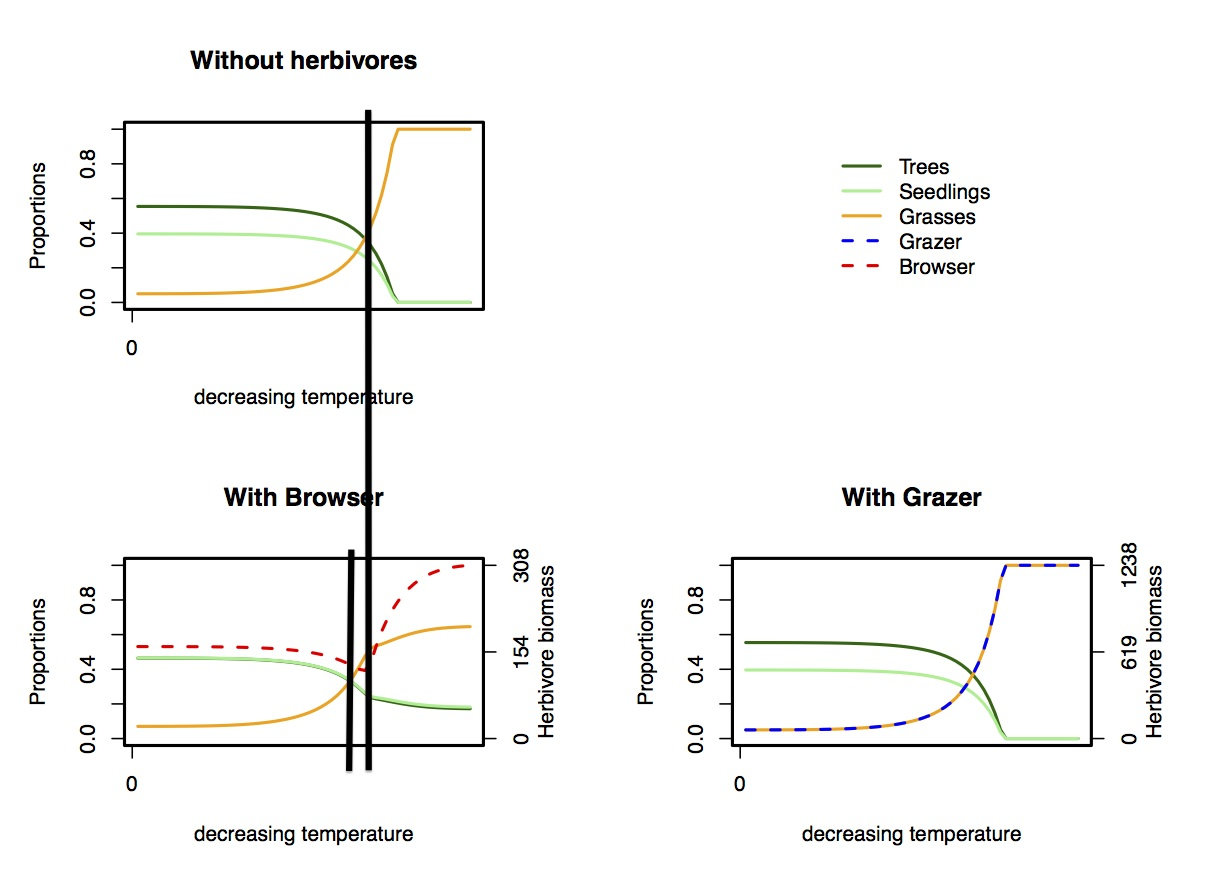
\includegraphics[width=0.8\textwidth]{../../ThreeSTModel/graphs/effectOnVeget_compare2.jpg}
}

\only<3>{
Indirect interactions between herbivores
\centering
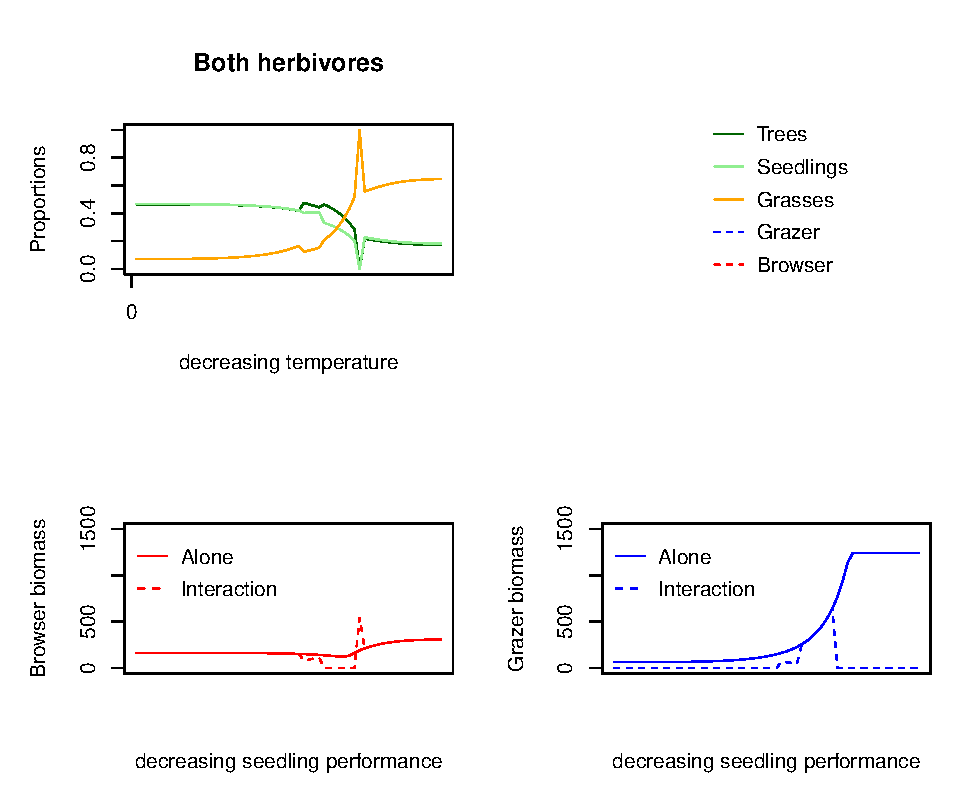
\includegraphics[width=0.8\textwidth]{../../ThreeSTModel/graphs/competition_facilitation.pdf}
}

% \only<4>{
% Importance of the feedback effect on the vegetation
% \centering
% 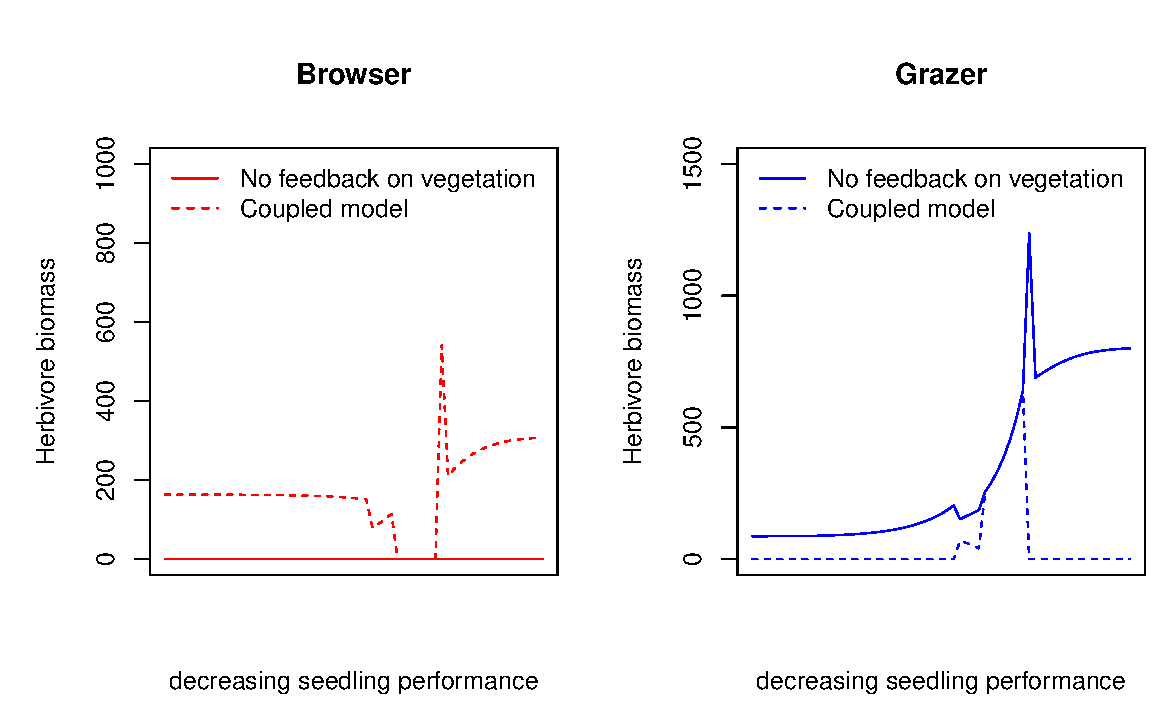
\includegraphics[width=0.8\textwidth]{../../ThreeSTModel/graphs/feedback_importance.pdf}
% }

% \only<5>{
% Effects along the gradient: summary
% \centering
% 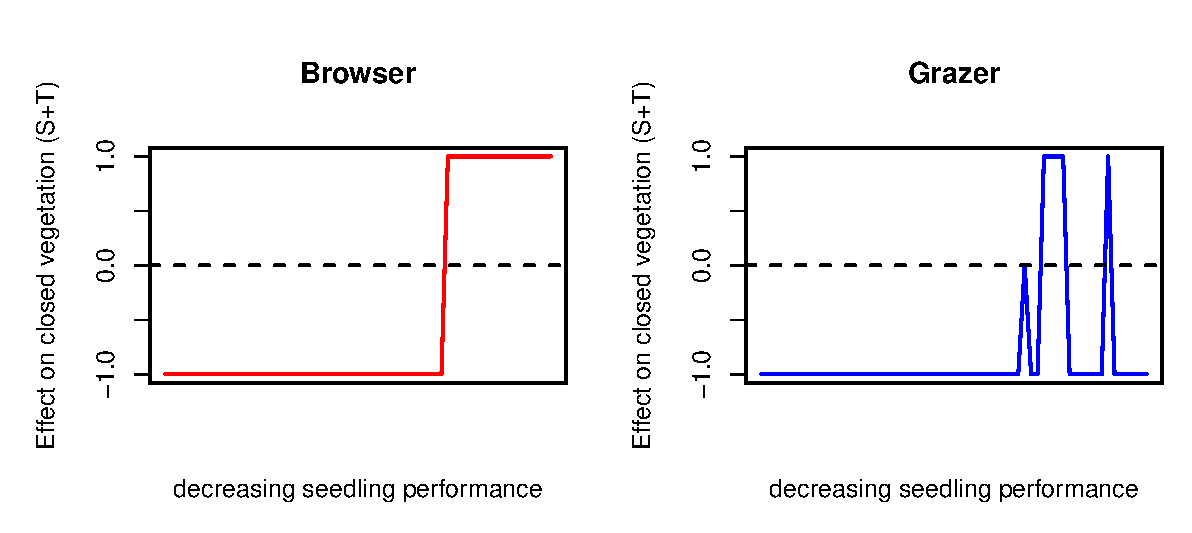
\includegraphics[height=0.4\textheight]{../../ThreeSTModel/graphs/effectOnVeget_sign_single.pdf}\\
% \centering
% 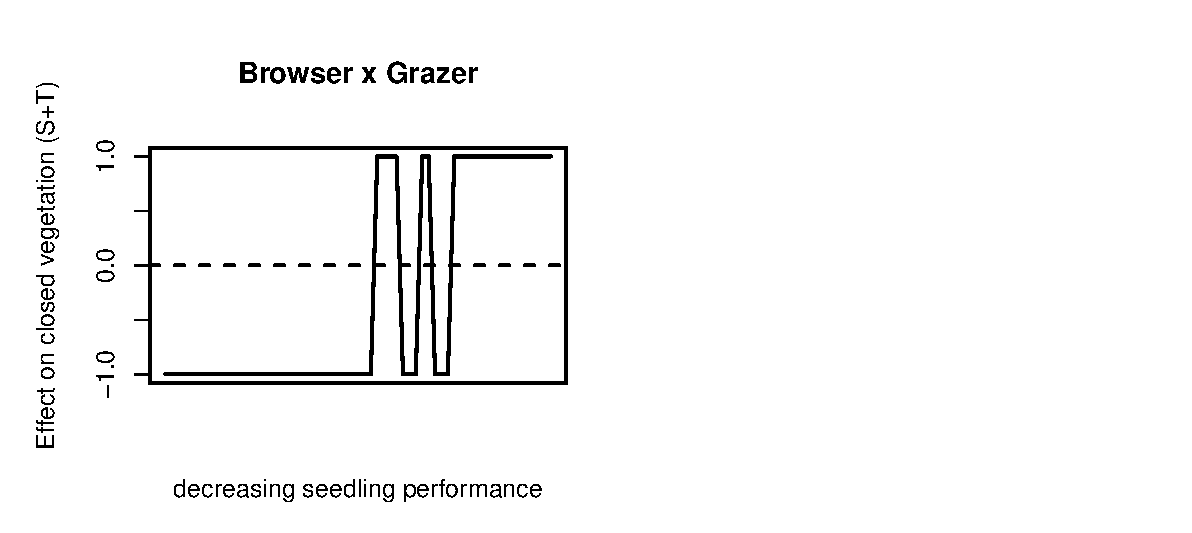
\includegraphics[height=0.4\textheight]{../../ThreeSTModel/graphs/effectOnVeget_sign_both.pdf}
% }


\end{frame}
%==========================================================================
%==========================================================================

\begin{frame}{Part 1: conclusions}
\begin{enumerate}

\item The herbivores induce a \alert{shift} in the distribution of the vegetation 

\item The herbivores \alert{modify the proportion} of vegetation states along the gradient
\begin{itemize}
\item The browser \alert{favors open environments where seedlings perform well}
\item The browser \alert{limits grasslands dominance where seedlings have low performance} 
\end{itemize}

% \item The feedback of herbivores on vegetation \alert{enhances their coexistence}

\item There are climatic conditions where \alert{indirect facilitation} between herbivores are more important than direct competition.

\end{enumerate}


\end{frame}
%==========================================================================
%==========================================================================

\begin{frame}[fragile]{Part 2: Temperate-boreal forest transition}

\begin{columns}
\begin{column}{0.5\textwidth}

$R$ = post-disturbance forest\\
$T$ = temperate forest\\

\end{column}
\begin{column}{0.5\textwidth}

$B$ = boreal forest\\
$M$ = mixed forest\\
\end{column}
\end{columns}


% \begin{columns}
% \begin{column}{0.5\textwidth}

% 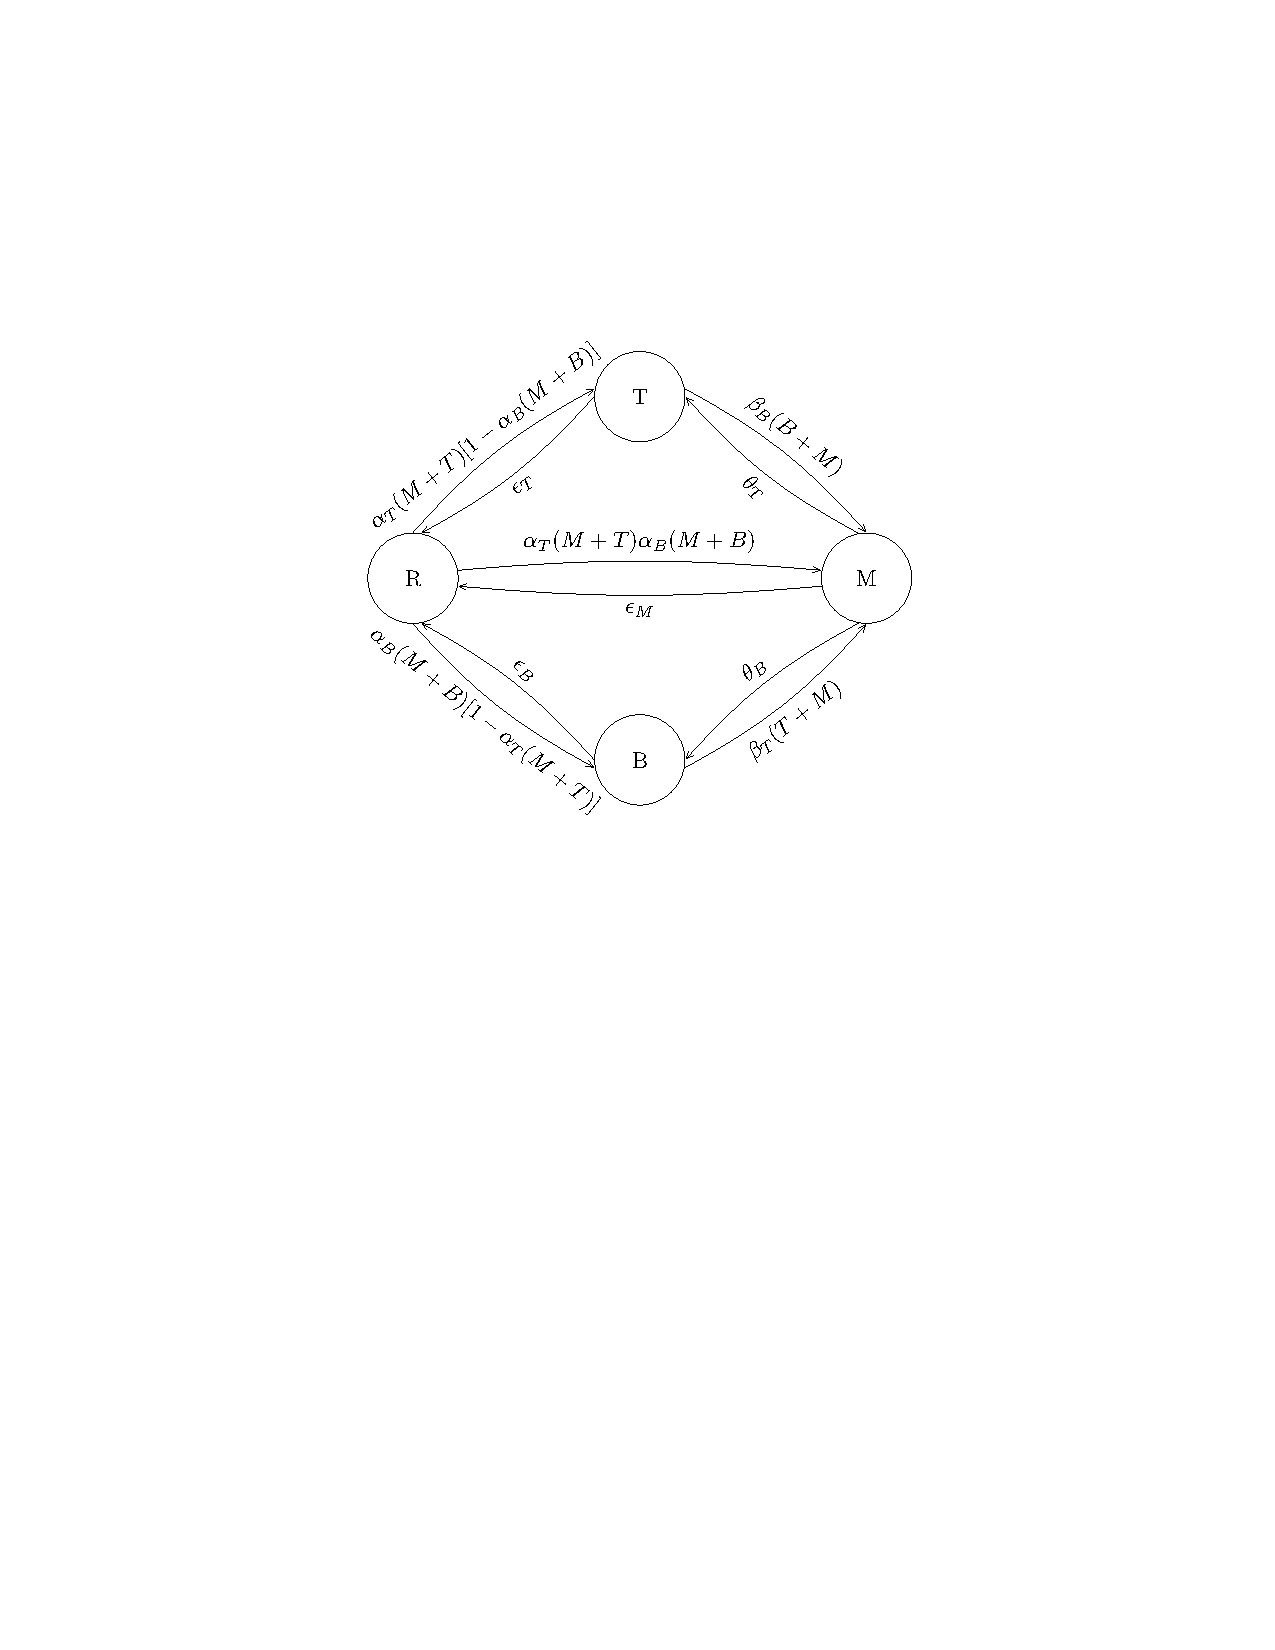
\includegraphics[width=\textwidth]{../../FourSTModel/graphiqueSTModel.pdf}

% \begin{tikzpicture}
% \matrix(m) [matrix of nodes, column sep=4em,
% 	row sep=3em,
% 	minimum width=2em,
% 	minimum height=2em,
% 	nodes={draw, circle, anchor=base}]
% 	{
% 	& \node[fill=tcolor!50]{T};  & \\
% 	\node[fill=orange!50]{R}; & & \node[fill=blue!50]{M}; \\
% 	& \node[fill=bcolor!50]{B}; & \\
% 	}; %end matrix

% \draw[-angle 45, draw=tcolor,ultra thick] (m-2-1.north) to[bend left=10] 
% node[midway,above, sloped] {\tiny{$\alpha_T(M+T)[1-\alpha_B(M+B)$}} (m-1-2.170) ;
% \draw[-angle 45,ultra thick] (m-1-2.west) to[bend left=10] 
% node[midway,below, sloped] {$\epsilon$} (m-2-1.80) ;

% \draw[-angle 45, draw = bcolor,ultra thick] (m-2-1.south) to[bend right=10] 
% node[midway,below, sloped] {\tiny{$\alpha_B(M+B)[1-\alpha_T(M+T)]$}} (m-3-2.190) ;
% \draw[-angle 45,ultra thick] (m-3-2.west) to[bend right=10] 
% node[midway,above, sloped] {$\epsilon$} (m-2-1.280) ;

% \draw[-angle 45,ultra thick, draw=blue] (m-2-1.10) to[bend left=5] 
% node[midway,above] {\tiny{$\alpha_T(M+T)\alpha_B(M+B)$}} (m-2-3.170) ;
% \draw[-angle 45,ultra thick] (m-2-3.190) to[bend left=5] 
% node[midway,below] {$\epsilon$} (m-2-1.350) ;

% \draw[-angle 45, draw=bcolor,ultra thick] (m-1-2.10) to[bend left=10] 
% node[midway,above, sloped] {\footnotesize{$\beta_B(B+M)$}} (m-2-3.north) ;
% \draw[-angle 45, draw=tcolor,ultra thick] (m-2-3.100) to[bend left=10] 
% node[midway,below, sloped] {$\theta_T$} (m-1-2.east) ;

% \draw[-angle 45, draw=tcolor,ultra thick] (m-3-2.350) to[bend right=10] 
% node[midway,below, sloped] {\footnotesize{$\beta_T(T+M)$}} (m-2-3.south) ;
% \draw[-angle 45, draw = bcolor,ultra thick] (m-2-3.260) to[bend right=10] 
% node[midway,above, sloped] {$\theta_B$} (m-3-2.east) ;

% \end{tikzpicture}
\centering
\begin{tikzpicture}
\matrix(m) [matrix of nodes, column sep=4em,
	row sep=3em,
	minimum width=2em,
	minimum height=2em,
	nodes={draw, circle, anchor=base}]
	{
	& \node[fill=tcolor!50]{T};  & \\
	\node[fill=orange!50]{R}; & & \node[fill=blue!50]{M}; \\
	& \node[fill=bcolor!50]{B}; & \\
	}; %end matrix

\draw[-angle 45, draw=tcolor,ultra thick] (m-2-1.north) to[bend left=10] 
node[midway,above, sloped] {regeneration} (m-1-2.170) ;
\draw[-angle 45,ultra thick] (m-1-2.west) to[bend left=10] 
node[midway,below, sloped] {disturbance} (m-2-1.80) ;

\draw[-angle 45, draw = bcolor,ultra thick] (m-2-1.south) to[bend right=10] 
node[midway,below, sloped] {regeneration} (m-3-2.190) ;
\draw[-angle 45,ultra thick] (m-3-2.west) to[bend right=10] 
node[midway,above, sloped] {disturbance} (m-2-1.280) ;

\draw[-angle 45,ultra thick, draw=blue] (m-2-1.10) to[bend left=5] 
node[midway,above] {regeneration} (m-2-3.170) ;
\draw[-angle 45,ultra thick] (m-2-3.190) to[bend left=5] 
node[midway,below] {disturbance} (m-2-1.350) ;

\draw[-angle 45, draw=bcolor,ultra thick] (m-1-2.10) to[bend left=10] 
node[midway,above, sloped] {colonisation} (m-2-3.north) ;
\draw[-angle 45, draw=tcolor,ultra thick] (m-2-3.100) to[bend left=10] 
node[midway,below, sloped] {succession} (m-1-2.east) ;

\draw[-angle 45, draw=tcolor,ultra thick] (m-3-2.350) to[bend right=10] 
node[midway,below, sloped] {colonisation} (m-2-3.south) ;
\draw[-angle 45, draw = bcolor,ultra thick] (m-2-3.260) to[bend right=10] 
node[midway,above, sloped] {succession} (m-3-2.east) ;

\end{tikzpicture}

% \end{column}
% \begin{column}{0.5\textwidth}

% \small{
% \flushleft
% $\alpha_B$, $\alpha_T$ are \alert{regeneration} probabilities %(related to seedling survival)

% $\beta_T$ and $\beta_B$ are \alert{colonisation} probabilities 

% $\theta_T$ and $\theta_B$ are \alert{competitive exclusion} probabilities in mixed forests

% $\epsilon$ are \alert{disturbances} probabilities
% }
% \end{column}
% \end{columns}
\end{frame}
%==========================================================================
%==========================================================================

\begin{frame}{Shelter effects}


% \textbf{Intakes}
% \[
% I = \overbrace{\frac{\tau F}{\mu+F}}^\text{intake rate of preferred resource} 
% + \overbrace{\frac{\rho G}{\nu+G}\Big(\phi + \frac{1-\phi}{ 1+e^{r(\frac{\tau F}{\mu+F} - p)}}}^\text{intake rate of secondary resource} \Big)
% \]
% \small{$\phi$ is the basal proportion of secondary resource used}
% \vspace{1em}

% \flushleft
% \textbf{Shelter effect}: 
The mortality dependents on the proportion of \alert{mature boreal and mixed} forests
% \begin{columns}
% \begin{column}{0.5\textwidth}

\centering
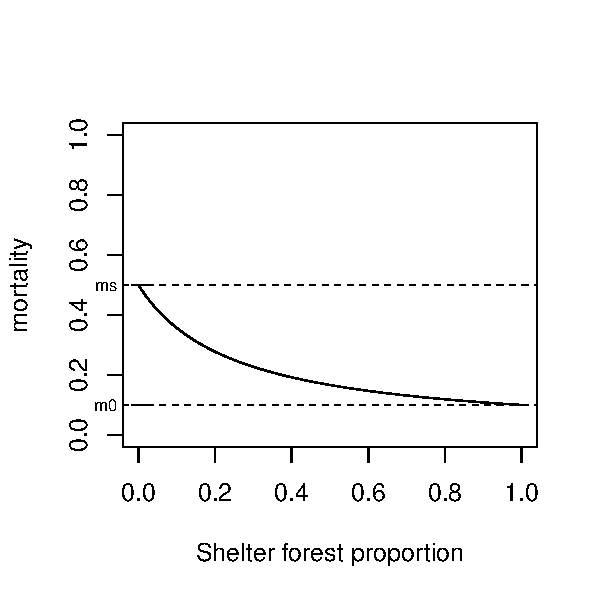
\includegraphics[width=0.4\textwidth]{../graphs/shelter_effect.pdf}
% \vspace{1em}
% \end{column}
% \begin{column}{0.5\textwidth}
% \[
% m = \frac{m_s}{(1+(\frac{m_s}{m_0}-1)(B+M))}
% \]
% \end{column}
% \end{columns}

\end{frame}
%==========================================================================
%==========================================================================
\begin{frame}[fragile]{Herbivore habitat and species preferences}


\begin{tikzpicture}
\matrix(m) [matrix of nodes, column sep=5em,
	row sep=2em,
	minimum width=2em,
	minimum height=2em,
	nodes={draw, anchor=base}]
	{
	& \node[rectangle]{Post disturbance forest}; & \node[circle, fill=orange!50]{R};\\
	\node[rectangle]{Habitat}; & & \node[circle, fill=tcolor!50]{T}; \\
	& \node[rectangle]{Mature forest}; & \node[circle, fill=bcolor!50]{B}; \\
	& & \node[circle, fill=blue!50]{M}; \\
	}; %end matrix

\draw[-angle 45, thick] (m-2-1.north) to node[midway,above, sloped] {} (m-1-2.west) ;
\draw[-angle 45, thick] (m-1-2.east) to (m-1-3.west) ;
\draw[-angle 45, thick] (m-2-1.south) to node[midway,above, sloped] {} (m-3-2.west) ;
\draw[-angle 45, thick] (m-3-2.north) to node[midway,above, sloped] {} (m-2-3.west) ;
\draw[-angle 45, thick] (m-3-2.east) to node[midway,above, sloped] {} (m-3-3.west) ;
\draw[-angle 45, thick] (m-3-2.south) to node[midway,above, sloped] {} (m-4-3.west) ;

\end{tikzpicture}

% \end{frame}
% %==========================================================================
% %==========================================================================

% \begin{frame}{Herbivore pressure on vegetation dynamics}


In each habitat, there is also species preferences ($\kappa_T$ and $\kappa_B$)


% \[
% P_{\text{seedling type}, \text{habitat type}} = \frac{\text{intakes}\times\text{habitat preference}\times\text{seedling impact}}{\text{habitat availability}}
% \]

% where $\text{seedling type}\in \{T, B\}$ \\
% and $\text{habitat type}\in \{T, B, R, M\}$

\end{frame}
%==========================================================================
%==========================================================================

\begin{frame}{Application in Québec}

\begin{columns}
\begin{column}{0.5\textwidth}

\onslide<1-2>{

\begin{enumerate}
\item Québec region

\onslide<2>{
\item Two competing browsers: 
\begin{itemize}
\item \textbf{White-tailed deer}. \\

\includegraphics[width=0.5\textwidth]{../../illustrations/deer.JPG}

\item \textbf{Moose}\\
\includegraphics[width=0.5\textwidth]{../../illustrations/moose.jpg}
}
\end{itemize}
}
\end{enumerate}

\end{column}
\begin{column}{0.5\textwidth}

\includegraphics[width=0.9\textwidth]{../../illustrations/models_acerQ.png}\\
\includegraphics[width=0.9\textwidth]{../../illustrations/legend_model_acer.png}\\
\centering
\tiny{\textit{Acer saccharum, Morin and Thuiller 2009}}



\end{column}
\end{columns}
\end{frame}
%==========================================================================
%==========================================================================

\begin{frame}{Parameterisation for herbivores and interactions}

\begin{columns}
\begin{column}{0.35\textwidth}

Data from literature:
\small{
\begin{itemize}

\item digestibility
\item habitat preferences
\item diet
\item metabolic rates
\item intake rates
\item home range size
\item distance travelled per day
\item forage availability

\end{itemize}
}
\end{column}
\begin{column}{0.65\textwidth}

\only<1>{
Deer carying capacity %(without feedbacks) versus observations
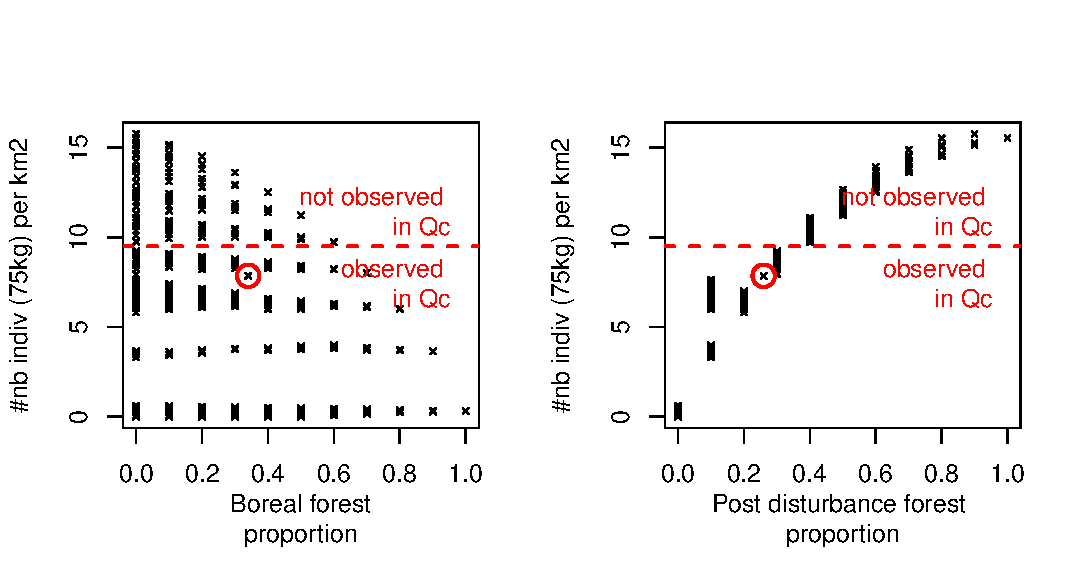
\includegraphics[width=\textwidth]{../graphs/validation_deer.pdf}\\
\centering
\includegraphics[width=0.4\textwidth]{../../illustrations/deer.JPG}

}
\only<2>{
Moose carying capacity %(without feedbacks) versus observations
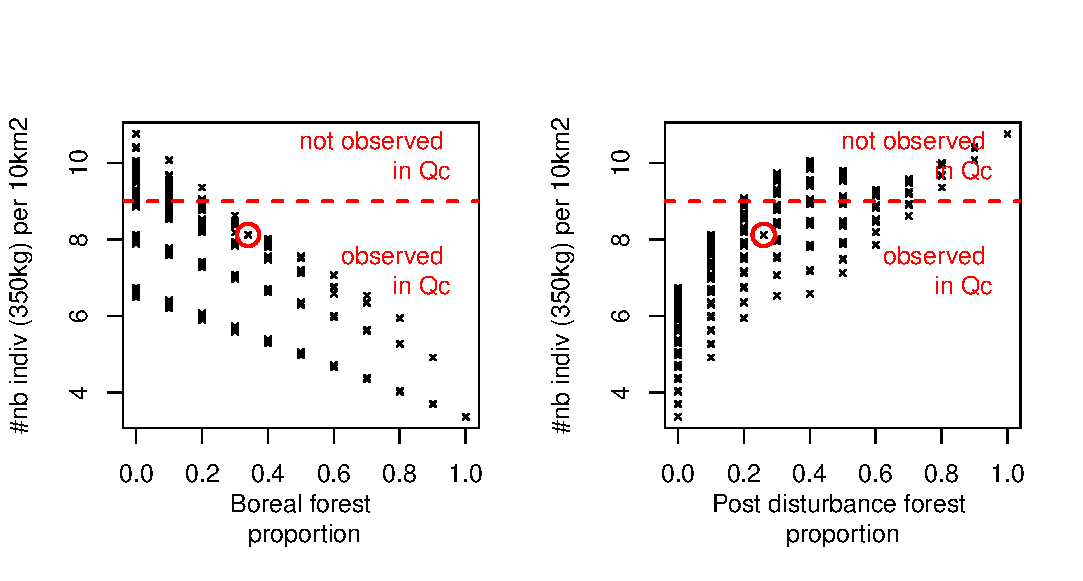
\includegraphics[width=\textwidth]{../graphs/validation_moose.pdf}\\
\centering
\includegraphics[width=0.4\textwidth]{../../illustrations/moose.jpg}

}

\end{column}
\end{columns}

\end{frame}

%==========================================================================
%==========================================================================

\begin{frame}{Parameterisation for vegetation}

Input data: 
\begin{itemize}
\item permanent plots (repeated measures of all trees >9cm dbh)
\item associated climatic data
\item moose and deer densities in whole Québec
\end{itemize}

\vspace{1em}

Parameter estimation:
\begin{itemize}
\item customized \alert{likelihood function}
\item \alert{simulated annealing} to estimate maximum likelihood
\end{itemize}

\end{frame}
%==========================================================================
%==========================================================================

\begin{frame}[fragile]{Estimated parameters}

\begin{columns}
\begin{column}{0.5\textwidth}

\begin{tikzpicture}
\matrix(m) [matrix of nodes, column sep=4em,
	row sep=3em,
	minimum width=2em,
	minimum height=2em,
	nodes={draw, circle, anchor=base}]
	{
	& \node[fill=tcolor!50]{T};  & \\
	\node[fill=orange!50]{R}; & & \node[fill=blue!50]{M}; \\
	& \node[fill=bcolor!50]{B}; & \\
	}; %end matrix

\draw[-angle 45, draw=tcolor,ultra thick] (m-2-1.north) to[bend left=10] 
node[midway,above, sloped] {regeneration} (m-1-2.170) ;
\draw[-angle 45,ultra thick] (m-1-2.west) to[bend left=10] 
node[midway,below, sloped] {disturbance} (m-2-1.80) ;

\draw[-angle 45, draw = bcolor,ultra thick] (m-2-1.south) to[bend right=10] 
node[midway,below, sloped] {regeneration} (m-3-2.190) ;
\draw[-angle 45,ultra thick] (m-3-2.west) to[bend right=10] 
node[midway,above, sloped] {disturbance} (m-2-1.280) ;

\draw[-angle 45,ultra thick, draw=blue] (m-2-1.10) to[bend left=5] 
node[midway,above] {regeneration} (m-2-3.170) ;
\draw[-angle 45,ultra thick] (m-2-3.190) to[bend left=5] 
node[midway,below] {disturbance} (m-2-1.350) ;

\draw[-angle 45, draw=bcolor,ultra thick] (m-1-2.10) to[bend left=10] 
node[midway,above, sloped] {colonisation} (m-2-3.north) ;
\draw[-angle 45, draw=tcolor,ultra thick] (m-2-3.100) to[bend left=10] 
node[midway,below, sloped] {succession} (m-1-2.east) ;

\draw[-angle 45, draw=tcolor,ultra thick] (m-3-2.350) to[bend right=10] 
node[midway,below, sloped] {colonisation} (m-2-3.south) ;
\draw[-angle 45, draw = bcolor,ultra thick] (m-2-3.260) to[bend right=10] 
node[midway,above, sloped] {succession} (m-3-2.east) ;

\end{tikzpicture}
\end{column}
\begin{column}{0.5\textwidth}


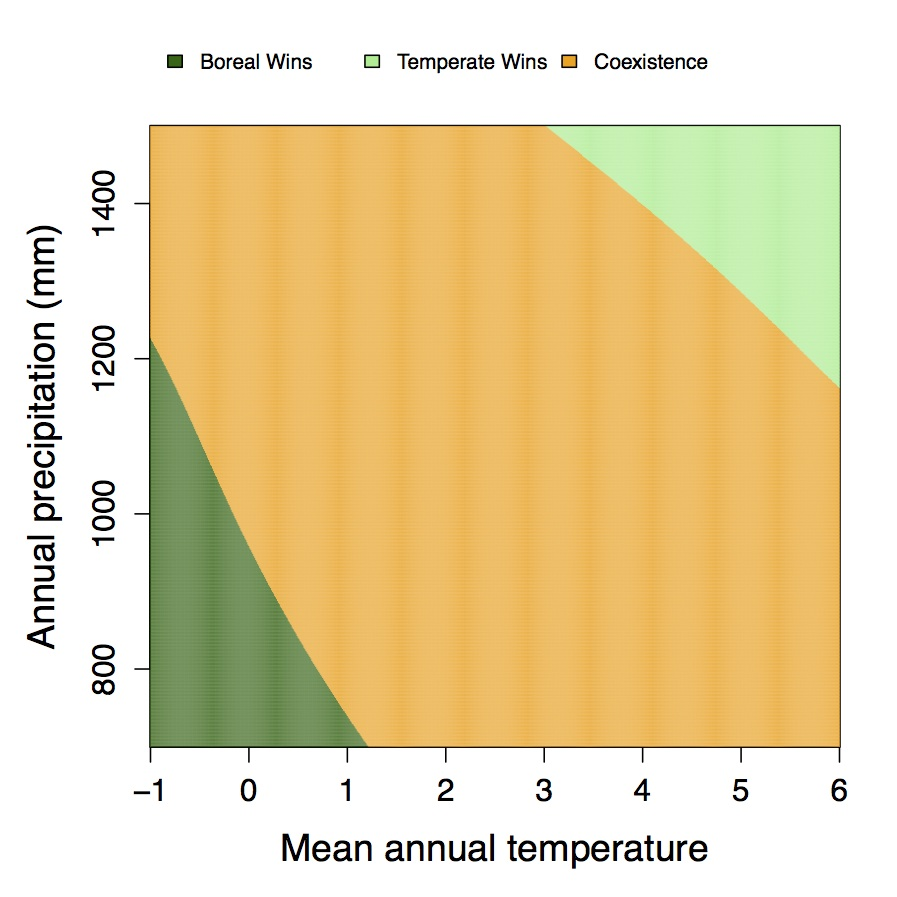
\includegraphics[width=\textwidth]{../fit_model_m3_ok/Coexistence_area.jpg}\\
\end{column}
\end{columns}

\end{frame}
%==========================================================================
%==========================================================================


\begin{frame}{Simulated climate change}

Simulated increase in 3\degre C in the vegetation coexistence zone.
\centering
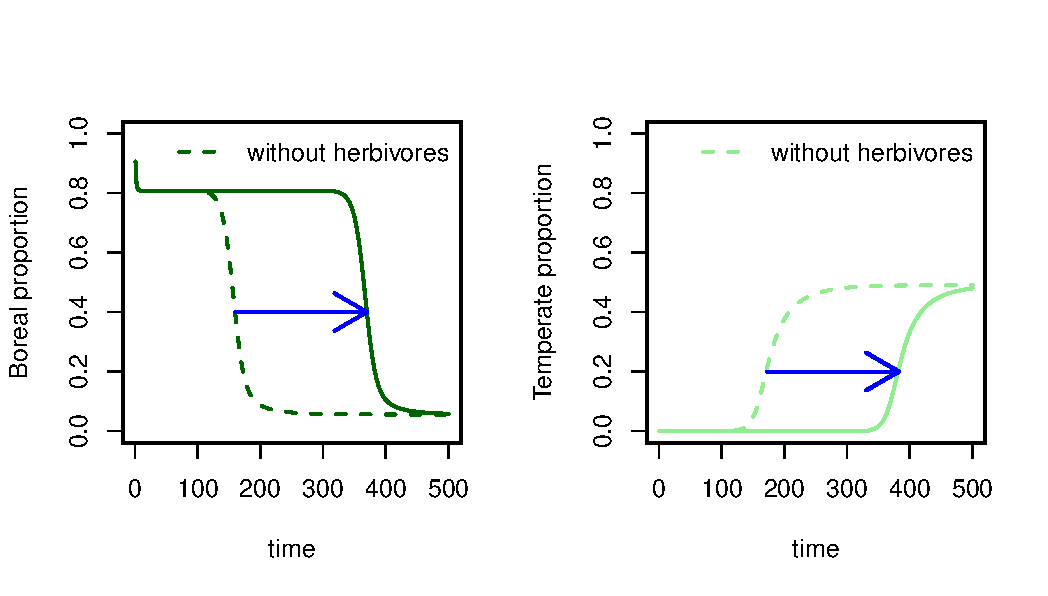
\includegraphics[width=0.8\textwidth]{../graphs/climate_change.pdf}\\


\end{frame}
%==========================================================================
%==========================================================================

% \begin{frame}{Part 2: conclusion}

% Herbivores may \alert{delay} the effect of climate change on the vegetation

% \end{frame}
%==========================================================================
%==========================================================================

\begin{frame}{Take home messages}

\begin{enumerate}

\item Herbivores can \alert{favor species coexistence} (for the 2 trophic levels)

\item Herbivores can induce a \alert{shift} in vegetation distributions 

\item Herbivores can \alert{delay} the effect of climate change on the vegetation

\end{enumerate}

\end{frame}
%==========================================================================
%==========================================================================
% \begin{frame}[plain]
% % \hspace*{-0pt}
% \makebox[\linewidth][c]{%
% \includegraphics[width=\paperwidth]{../presentations_figs/questions.pdf}
% }
% \end{frame}


%==========================================================================

\end{document}
